\documentclass[1p]{elsarticle_modified}
%\bibliographystyle{elsarticle-num}

%\usepackage[colorlinks]{hyperref}
%\usepackage{abbrmath_seonhwa} %\Abb, \Ascr, \Acal ,\Abf, \Afrak
\usepackage{amsfonts}
\usepackage{amssymb}
\usepackage{amsmath}
\usepackage{amsthm}
\usepackage{scalefnt}
\usepackage{amsbsy}
\usepackage{kotex}
\usepackage{caption}
\usepackage{subfig}
\usepackage{color}
\usepackage{graphicx}
\usepackage{xcolor} %% white, black, red, green, blue, cyan, magenta, yellow
\usepackage{float}
\usepackage{setspace}
\usepackage{hyperref}

\usepackage{tikz}
\usetikzlibrary{arrows}

\usepackage{multirow}
\usepackage{array} % fixed length table
\usepackage{hhline}

%%%%%%%%%%%%%%%%%%%%%
\makeatletter
\renewcommand*\env@matrix[1][\arraystretch]{%
	\edef\arraystretch{#1}%
	\hskip -\arraycolsep
	\let\@ifnextchar\new@ifnextchar
	\array{*\c@MaxMatrixCols c}}
\makeatother %https://tex.stackexchange.com/questions/14071/how-can-i-increase-the-line-spacing-in-a-matrix
%%%%%%%%%%%%%%%

\usepackage[normalem]{ulem}

\newcommand{\msout}[1]{\ifmmode\text{\sout{\ensuremath{#1}}}\else\sout{#1}\fi}
%SOURCE: \msout is \stkout macro in https://tex.stackexchange.com/questions/20609/strikeout-in-math-mode

\newcommand{\cancel}[1]{
	\ifmmode
	{\color{red}\msout{#1}}
	\else
	{\color{red}\sout{#1}}
	\fi
}

\newcommand{\add}[1]{
	{\color{blue}\uwave{#1}}
}

\newcommand{\replace}[2]{
	\ifmmode
	{\color{red}\msout{#1}}{\color{blue}\uwave{#2}}
	\else
	{\color{red}\sout{#1}}{\color{blue}\uwave{#2}}
	\fi
}

\newcommand{\Sol}{\mathcal{S}} %segment
\newcommand{\D}{D} %diagram
\newcommand{\A}{\mathcal{A}} %arc


%%%%%%%%%%%%%%%%%%%%%%%%%%%%%5 test

\def\sl{\operatorname{\textup{SL}}(2,\Cbb)}
\def\psl{\operatorname{\textup{PSL}}(2,\Cbb)}
\def\quan{\mkern 1mu \triangleright \mkern 1mu}

\theoremstyle{definition}
\newtheorem{thm}{Theorem}[section]
\newtheorem{prop}[thm]{Proposition}
\newtheorem{lem}[thm]{Lemma}
\newtheorem{ques}[thm]{Question}
\newtheorem{cor}[thm]{Corollary}
\newtheorem{defn}[thm]{Definition}
\newtheorem{exam}[thm]{Example}
\newtheorem{rmk}[thm]{Remark}
\newtheorem{alg}[thm]{Algorithm}

\newcommand{\I}{\sqrt{-1}}
\begin{document}

%\begin{frontmatter}
%
%\title{Boundary parabolic representations of knots up to 8 crossings}
%
%%% Group authors per affiliation:
%\author{Yunhi Cho} 
%\address{Department of Mathematics, University of Seoul, Seoul, Korea}
%\ead{yhcho@uos.ac.kr}
%
%
%\author{Seonhwa Kim} %\fnref{s_kim}}
%\address{Center for Geometry and Physics, Institute for Basic Science, Pohang, 37673, Korea}
%\ead{ryeona17@ibs.re.kr}
%
%\author{Hyuk Kim}
%\address{Department of Mathematical Sciences, Seoul National University, Seoul 08826, Korea}
%\ead{hyukkim@snu.ac.kr}
%
%\author{Seokbeom Yoon}
%\address{Department of Mathematical Sciences, Seoul National University, Seoul, 08826,  Korea}
%\ead{sbyoon15@snu.ac.kr}
%
%\begin{abstract}
%We find all boundary parabolic representation of knots up to 8 crossings.
%
%\end{abstract}
%\begin{keyword}
%    \MSC[2010] 57M25 
%\end{keyword}
%
%\end{frontmatter}

%\linenumbers
%\tableofcontents
%
\newcommand\colored[1]{\textcolor{white}{\rule[-0.35ex]{0.8em}{1.4ex}}\kern-0.8em\color{red} #1}%
%\newcommand\colored[1]{\textcolor{white}{ #1}\kern-2.17ex	\textcolor{white}{ #1}\kern-1.81ex	\textcolor{white}{ #1}\kern-2.15ex\color{red}#1	}

{\Large $\underline{12n_{0543}~(K12n_{0543})}$}

\setlength{\tabcolsep}{10pt}
\renewcommand{\arraystretch}{1.6}
\vspace{1cm}\begin{tabular}{m{100pt}>{\centering\arraybackslash}m{274pt}}
\multirow{5}{120pt}{
	\centering
	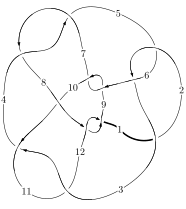
\includegraphics[width=112pt]{../../../GIT/diagram.site/Diagrams/png/2632_12n_0543.png}\\
\ \ \ A knot diagram\footnotemark}&
\allowdisplaybreaks
\textbf{Linearized knot diagam} \\
\cline{2-2}
 &
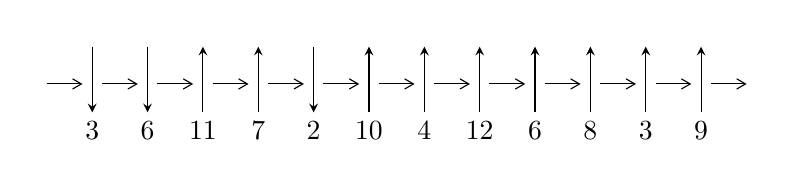
\begin{tikzpicture}[x=20pt, y=17pt]
	% nodes
	\node (C0) at (0, 0) {};
	\node (C1) at (1, 0) {};
	\node (C1U) at (1, +1) {};
	\node (C1D) at (1, -1) {3};

	\node (C2) at (2, 0) {};
	\node (C2U) at (2, +1) {};
	\node (C2D) at (2, -1) {6};

	\node (C3) at (3, 0) {};
	\node (C3U) at (3, +1) {};
	\node (C3D) at (3, -1) {11};

	\node (C4) at (4, 0) {};
	\node (C4U) at (4, +1) {};
	\node (C4D) at (4, -1) {7};

	\node (C5) at (5, 0) {};
	\node (C5U) at (5, +1) {};
	\node (C5D) at (5, -1) {2};

	\node (C6) at (6, 0) {};
	\node (C6U) at (6, +1) {};
	\node (C6D) at (6, -1) {10};

	\node (C7) at (7, 0) {};
	\node (C7U) at (7, +1) {};
	\node (C7D) at (7, -1) {4};

	\node (C8) at (8, 0) {};
	\node (C8U) at (8, +1) {};
	\node (C8D) at (8, -1) {12};

	\node (C9) at (9, 0) {};
	\node (C9U) at (9, +1) {};
	\node (C9D) at (9, -1) {6};

	\node (C10) at (10, 0) {};
	\node (C10U) at (10, +1) {};
	\node (C10D) at (10, -1) {8};

	\node (C11) at (11, 0) {};
	\node (C11U) at (11, +1) {};
	\node (C11D) at (11, -1) {3};

	\node (C12) at (12, 0) {};
	\node (C12U) at (12, +1) {};
	\node (C12D) at (12, -1) {9};
	\node (C13) at (13, 0) {};

	% arrows
	\draw[->,>={angle 60}]
	(C0) edge (C1) (C1) edge (C2) (C2) edge (C3) (C3) edge (C4) (C4) edge (C5) (C5) edge (C6) (C6) edge (C7) (C7) edge (C8) (C8) edge (C9) (C9) edge (C10) (C10) edge (C11) (C11) edge (C12) (C12) edge (C13) ;	\draw[->,>=stealth]
	(C1U) edge (C1D) (C2U) edge (C2D) (C3D) edge (C3U) (C4D) edge (C4U) (C5U) edge (C5D) (C6D) edge (C6U) (C7D) edge (C7U) (C8D) edge (C8U) (C9D) edge (C9U) (C10D) edge (C10U) (C11D) edge (C11U) (C12D) edge (C12U) ;
	\end{tikzpicture} \\
\hhline{~~} \\& 
\textbf{Solving Sequence} \\ \cline{2-2} 
 &
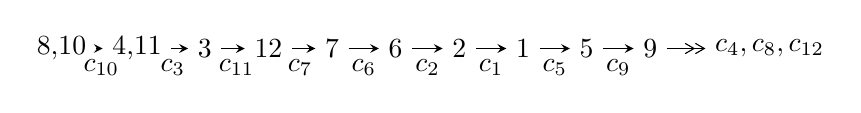
\begin{tikzpicture}[x=23pt, y=7pt]
	% node
	\node (A0) at (-1/8, 0) {8,10};
	\node (A1) at (17/16, 0) {4,11};
	\node (A2) at (17/8, 0) {3};
	\node (A3) at (25/8, 0) {12};
	\node (A4) at (33/8, 0) {7};
	\node (A5) at (41/8, 0) {6};
	\node (A6) at (49/8, 0) {2};
	\node (A7) at (57/8, 0) {1};
	\node (A8) at (65/8, 0) {5};
	\node (A9) at (73/8, 0) {9};
	\node (C1) at (1/2, -1) {$c_{10}$};
	\node (C2) at (13/8, -1) {$c_{3}$};
	\node (C3) at (21/8, -1) {$c_{11}$};
	\node (C4) at (29/8, -1) {$c_{7}$};
	\node (C5) at (37/8, -1) {$c_{6}$};
	\node (C6) at (45/8, -1) {$c_{2}$};
	\node (C7) at (53/8, -1) {$c_{1}$};
	\node (C8) at (61/8, -1) {$c_{5}$};
	\node (C9) at (69/8, -1) {$c_{9}$};
	\node (A10) at (11, 0) {$c_{4},c_{8},c_{12}$};

	% edge
	\draw[->,>=stealth]	
	(A0) edge (A1) (A1) edge (A2) (A2) edge (A3) (A3) edge (A4) (A4) edge (A5) (A5) edge (A6) (A6) edge (A7) (A7) edge (A8) (A8) edge (A9) ;
	\draw[->>,>={angle 60}]	
	(A9) edge (A10);
\end{tikzpicture} \\ 

\end{tabular} \\

\footnotetext{
The image of knot diagram is generated by the software ``\textbf{Draw programme}" developed by Andrew Bartholomew(\url{http://www.layer8.co.uk/maths/draw/index.htm\#Running-draw}), where we modified some parts for our purpose(\url{https://github.com/CATsTAILs/LinksPainter}).
}\phantom \\ \newline 
\centering \textbf{Ideals for irreducible components\footnotemark of $X_{\text{par}}$} 
 
\begin{align*}
I^u_{1}&=\langle 
-7700 u^{17}+5343 u^{16}+\cdots+94946 b-375396,\\
\phantom{I^u_{1}}&\phantom{= \langle  }-208501 u^{17}-1574159 u^{16}+\cdots+189892 a-47374,\;u^{18}+9 u^{17}+\cdots-32 u-8\rangle \\
I^u_{2}&=\langle 
2 u^{15}-8 u^{14}+\cdots+4 b-3,\;-3 u^{15} a- u^{15}+\cdots+4 a-5,\\
\phantom{I^u_{2}}&\phantom{= \langle  }u^{16}-5 u^{15}+13 u^{14}-20 u^{13}+20 u^{12}-13 u^{11}+7 u^{10}-4 u^9+5 u^8-6 u^7+7 u^6+u^5+u^3+2 u^2-2 u+1\rangle \\
I^u_{3}&=\langle 
u^5- u^4+4 u^2+b-3 u+1,\;u^6+4 u^3+u^2+a+u,\;u^7-2 u^6+2 u^5+3 u^4-7 u^3+7 u^2-4 u+1\rangle \\
I^u_{4}&=\langle 
u^2+b-1,\;- u^2+a+u,\;u^4- u^2+1\rangle \\
I^u_{5}&=\langle 
u^2+b-2 u,\;- u^3+3 u^2+a-2 u-1,\;u^4-4 u^3+5 u^2-2 u+1\rangle \\
I^u_{6}&=\langle 
- u^3+b+1,\;u^2+a,\;u^4- u^2+1\rangle \\
\\
\end{align*}
\raggedright * 6 irreducible components of $\dim_{\mathbb{C}}=0$, with total 69 representations.\\
\footnotetext{All coefficients of polynomials are rational numbers. But the coefficients are sometimes approximated in decimal forms when there is not enough margin.}
\newpage
\renewcommand{\arraystretch}{1}
\centering \section*{I. $I^u_{1}= \langle -7700 u^{17}+5343 u^{16}+\cdots+94946 b-375396,\;-2.09\times10^{5} u^{17}-1.57\times10^{6} u^{16}+\cdots+1.90\times10^{5} a-4.74\times10^{4},\;u^{18}+9 u^{17}+\cdots-32 u-8 \rangle$}
\flushleft \textbf{(i) Arc colorings}\\
\begin{tabular}{m{7pt} m{180pt} m{7pt} m{180pt} }
\flushright $a_{8}=$&$\begin{pmatrix}0\\u\end{pmatrix}$ \\
\flushright $a_{10}=$&$\begin{pmatrix}1\\0\end{pmatrix}$ \\
\flushright $a_{4}=$&$\begin{pmatrix}1.09800 u^{17}+8.28976 u^{16}+\cdots-15.7165 u+0.249479\\0.0810987 u^{17}-0.0562741 u^{16}+\cdots+6.78168 u+3.95378\end{pmatrix}$ \\
\flushright $a_{11}=$&$\begin{pmatrix}1\\- u^2\end{pmatrix}$ \\
\flushright $a_{3}=$&$\begin{pmatrix}-0.494223 u^{17}-4.52911 u^{16}+\cdots+19.6689 u+9.03346\\0.806058 u^{17}+7.39600 u^{16}+\cdots-28.8365 u-8.13519\end{pmatrix}$ \\
\flushright $a_{12}=$&$\begin{pmatrix}-1.22543 u^{17}-10.2441 u^{16}+\cdots+36.7104 u+11.2034\\-0.156958 u^{17}-1.34093 u^{16}+\cdots+11.8068 u+6.16152\end{pmatrix}$ \\
\flushright $a_{7}=$&$\begin{pmatrix}1.55492 u^{17}+13.6648 u^{16}+\cdots-63.8250 u-22.6427\\0.784725 u^{17}+6.89000 u^{16}+\cdots-28.0103 u-9.80343\end{pmatrix}$ \\
\flushright $a_{6}=$&$\begin{pmatrix}0.770190 u^{17}+6.77476 u^{16}+\cdots-35.8147 u-12.8393\\0.784725 u^{17}+6.89000 u^{16}+\cdots-28.0103 u-9.80343\end{pmatrix}$ \\
\flushright $a_{2}=$&$\begin{pmatrix}0.290215 u^{17}+2.16110 u^{16}+\cdots+2.43279 u+1.45741\\-0.157274 u^{17}-1.91408 u^{16}+\cdots+16.4252 u+6.18248\end{pmatrix}$ \\
\flushright $a_{1}=$&$\begin{pmatrix}2.34412 u^{17}+18.5078 u^{16}+\cdots-50.0957 u-13.4097\\-1.64756 u^{17}-13.1645 u^{16}+\cdots+21.7849 u+2.78798\end{pmatrix}$ \\
\flushright $a_{5}=$&$\begin{pmatrix}2.10179 u^{17}+17.6337 u^{16}+\cdots-59.4695 u-17.2935\\-0.157274 u^{17}-1.91408 u^{16}+\cdots+16.4252 u+6.18248\end{pmatrix}$ \\
\flushright $a_{9}=$&$\begin{pmatrix}0.321980 u^{17}+2.64919 u^{16}+\cdots-15.1353 u-5.98303\\-0.248631 u^{17}-1.59965 u^{16}+\cdots+4.32034 u+2.57584\end{pmatrix}$\\&\end{tabular}
\flushleft \textbf{(ii) Obstruction class $= -1$}\\~\\
\flushleft \textbf{(iii) Cusp Shapes $= -\frac{296580}{47473} u^{17}-\frac{2538267}{47473} u^{16}+\cdots+\frac{10665772}{47473} u+\frac{3817158}{47473}$}\\~\\
\newpage\renewcommand{\arraystretch}{1}
\flushleft \textbf{(iv) u-Polynomials at the component}\newline \\
\begin{tabular}{m{50pt}|m{274pt}}
Crossings & \hspace{64pt}u-Polynomials at each crossing \\
\hline $$\begin{aligned}c_{1}\end{aligned}$$&$\begin{aligned}
&u^{18}+13 u^{17}+\cdots+12928 u+256
\end{aligned}$\\
\hline $$\begin{aligned}c_{2},c_{5}\end{aligned}$$&$\begin{aligned}
&u^{18}+11 u^{17}+\cdots-32 u+16
\end{aligned}$\\
\hline $$\begin{aligned}c_{3},c_{4},c_{7}\\c_{11}\end{aligned}$$&$\begin{aligned}
&u^{18}+u^{17}+\cdots-6 u+1
\end{aligned}$\\
\hline $$\begin{aligned}c_{6},c_{8},c_{9}\\c_{12}\end{aligned}$$&$\begin{aligned}
&u^{18}+u^{17}+\cdots-3 u-1
\end{aligned}$\\
\hline $$\begin{aligned}c_{10}\end{aligned}$$&$\begin{aligned}
&u^{18}+9 u^{17}+\cdots-32 u-8
\end{aligned}$\\
\hline
\end{tabular}\\~\\
\newpage\renewcommand{\arraystretch}{1}
\flushleft \textbf{(v) Riley Polynomials at the component}\newline \\
\begin{tabular}{m{50pt}|m{274pt}}
Crossings & \hspace{64pt}Riley Polynomials at each crossing \\
\hline $$\begin{aligned}c_{1}\end{aligned}$$&$\begin{aligned}
&y^{18}-25 y^{17}+\cdots-151904256 y+65536
\end{aligned}$\\
\hline $$\begin{aligned}c_{2},c_{5}\end{aligned}$$&$\begin{aligned}
&y^{18}-13 y^{17}+\cdots-12928 y+256
\end{aligned}$\\
\hline $$\begin{aligned}c_{3},c_{4},c_{7}\\c_{11}\end{aligned}$$&$\begin{aligned}
&y^{18}+17 y^{17}+\cdots-14 y+1
\end{aligned}$\\
\hline $$\begin{aligned}c_{6},c_{8},c_{9}\\c_{12}\end{aligned}$$&$\begin{aligned}
&y^{18}+3 y^{17}+\cdots- y+1
\end{aligned}$\\
\hline $$\begin{aligned}c_{10}\end{aligned}$$&$\begin{aligned}
&y^{18}-5 y^{17}+\cdots-416 y+64
\end{aligned}$\\
\hline
\end{tabular}\\~\\
\newpage\flushleft \textbf{(vi) Complex Volumes and Cusp Shapes}
$$\begin{array}{c|c|c}  
\text{Solutions to }I^u_{1}& \I (\text{vol} + \sqrt{-1}CS) & \text{Cusp shape}\\
 \hline 
\begin{aligned}
u &= -0.620829 + 0.451049 I \\
a &= -1.057030 - 0.908608 I \\
b &= -0.364836 - 0.513954 I\end{aligned}
 & -4.27022 - 1.76048 I & \phantom{-}4.57169 + 3.79716 I \\ \hline\begin{aligned}
u &= -0.620829 - 0.451049 I \\
a &= -1.057030 + 0.908608 I \\
b &= -0.364836 + 0.513954 I\end{aligned}
 & -4.27022 + 1.76048 I & \phantom{-}4.57169 - 3.79716 I \\ \hline\begin{aligned}
u &= \phantom{-}0.299337 + 0.584940 I \\
a &= -1.029310 - 0.829653 I \\
b &= -0.727675 + 1.001360 I\end{aligned}
 & -1.45016 + 2.06579 I & -1.19192 - 3.00311 I \\ \hline\begin{aligned}
u &= \phantom{-}0.299337 - 0.584940 I \\
a &= -1.029310 + 0.829653 I \\
b &= -0.727675 - 1.001360 I\end{aligned}
 & -1.45016 - 2.06579 I & -1.19192 + 3.00311 I \\ \hline\begin{aligned}
u &= -0.550550 + 0.319324 I \\
a &= \phantom{-}1.76918 - 0.57363 I \\
b &= \phantom{-}0.636691 - 0.143319 I\end{aligned}
 & \phantom{-}0.60964 - 2.63332 I & \phantom{-}1.40533 + 10.85901 I \\ \hline\begin{aligned}
u &= -0.550550 - 0.319324 I \\
a &= \phantom{-}1.76918 + 0.57363 I \\
b &= \phantom{-}0.636691 + 0.143319 I\end{aligned}
 & \phantom{-}0.60964 + 2.63332 I & \phantom{-}1.40533 - 10.85901 I \\ \hline\begin{aligned}
u &= \phantom{-}1.39562 + 0.46679 I \\
a &= \phantom{-}0.039259 + 0.359476 I \\
b &= \phantom{-}0.513460 - 1.193020 I\end{aligned}
 & \phantom{-}1.25038 + 1.91482 I & \phantom{-}14.6915 - 3.0336 I \\ \hline\begin{aligned}
u &= \phantom{-}1.39562 - 0.46679 I \\
a &= \phantom{-}0.039259 - 0.359476 I \\
b &= \phantom{-}0.513460 + 1.193020 I\end{aligned}
 & \phantom{-}1.25038 - 1.91482 I & \phantom{-}14.6915 + 3.0336 I \\ \hline\begin{aligned}
u &= -1.50565\phantom{ +0.000000I} \\
a &= \phantom{-}0.258519\phantom{ +0.000000I} \\
b &= -0.196820\phantom{ +0.000000I}\end{aligned}
 & \phantom{-}7.31535\phantom{ +0.000000I} & \phantom{-}30.1030\phantom{ +0.000000I} \\ \hline\begin{aligned}
u &= \phantom{-}0.460925\phantom{ +0.000000I} \\
a &= -0.513715\phantom{ +0.000000I} \\
b &= \phantom{-}0.345924\phantom{ +0.000000I}\end{aligned}
 & \phantom{-}0.812221\phantom{ +0.000000I} & \phantom{-}12.1610\phantom{ +0.000000I}\\
 \hline 
 \end{array}$$\newpage$$\begin{array}{c|c|c}  
\text{Solutions to }I^u_{1}& \I (\text{vol} + \sqrt{-1}CS) & \text{Cusp shape}\\
 \hline 
\begin{aligned}
u &= -0.99486 + 1.19077 I \\
a &= -0.774071 + 0.517855 I \\
b &= -1.71185 - 0.17534 I\end{aligned}
 & -7.59215 - 0.44788 I & \phantom{-}1.54300 - 0.72825 I \\ \hline\begin{aligned}
u &= -0.99486 - 1.19077 I \\
a &= -0.774071 - 0.517855 I \\
b &= -1.71185 + 0.17534 I\end{aligned}
 & -7.59215 + 0.44788 I & \phantom{-}1.54300 + 0.72825 I \\ \hline\begin{aligned}
u &= -1.13905 + 1.08250 I \\
a &= \phantom{-}0.869148 - 0.562899 I \\
b &= \phantom{-}1.65960 + 0.63204 I\end{aligned}
 & -7.10236 - 7.75507 I & \phantom{-}1.99474 + 5.37139 I \\ \hline\begin{aligned}
u &= -1.13905 - 1.08250 I \\
a &= \phantom{-}0.869148 + 0.562899 I \\
b &= \phantom{-}1.65960 - 0.63204 I\end{aligned}
 & -7.10236 + 7.75507 I & \phantom{-}1.99474 - 5.37139 I \\ \hline\begin{aligned}
u &= -1.13411 + 1.20889 I \\
a &= -0.943992 + 0.426963 I \\
b &= -1.89059 - 0.88824 I\end{aligned}
 & -14.6094 - 14.6374 I & \phantom{-}2.41427 + 6.49796 I \\ \hline\begin{aligned}
u &= -1.13411 - 1.20889 I \\
a &= -0.943992 - 0.426963 I \\
b &= -1.89059 + 0.88824 I\end{aligned}
 & -14.6094 + 14.6374 I & \phantom{-}2.41427 - 6.49796 I \\ \hline\begin{aligned}
u &= -1.23320 + 1.28187 I \\
a &= \phantom{-}0.504423 - 0.599474 I \\
b &= \phantom{-}1.81064 + 0.13552 I\end{aligned}
 & -14.4902 + 5.6411 I & \phantom{-}1.43945 - 2.69512 I \\ \hline\begin{aligned}
u &= -1.23320 - 1.28187 I \\
a &= \phantom{-}0.504423 + 0.599474 I \\
b &= \phantom{-}1.81064 - 0.13552 I\end{aligned}
 & -14.4902 - 5.6411 I & \phantom{-}1.43945 + 2.69512 I\\
 \hline 
 \end{array}$$\newpage\newpage\renewcommand{\arraystretch}{1}
\centering \section*{II. $I^u_{2}= \langle 2 u^{15}-8 u^{14}+\cdots+4 b-3,\;-3 u^{15} a- u^{15}+\cdots+4 a-5,\;u^{16}-5 u^{15}+\cdots-2 u+1 \rangle$}
\flushleft \textbf{(i) Arc colorings}\\
\begin{tabular}{m{7pt} m{180pt} m{7pt} m{180pt} }
\flushright $a_{8}=$&$\begin{pmatrix}0\\u\end{pmatrix}$ \\
\flushright $a_{10}=$&$\begin{pmatrix}1\\0\end{pmatrix}$ \\
\flushright $a_{4}=$&$\begin{pmatrix}a\\-\frac{1}{2} u^{15}+2 u^{14}+\cdots-\frac{1}{2} u+\frac{3}{4}\end{pmatrix}$ \\
\flushright $a_{11}=$&$\begin{pmatrix}1\\- u^2\end{pmatrix}$ \\
\flushright $a_{3}=$&$\begin{pmatrix}\frac{1}{2} u^{15}-2 u^{14}+\cdots+a-\frac{3}{4}\\-\frac{1}{2} u^{15}+\frac{9}{4} u^{14}+\cdots- u+\frac{5}{4}\end{pmatrix}$ \\
\flushright $a_{12}=$&$\begin{pmatrix}-\frac{1}{2} u^{15} a-\frac{7}{4} u^{15}+\cdots+\frac{1}{2} a+2\\\frac{1}{4} u^{15} a+\frac{3}{4} u^{15}+\cdots-\frac{1}{2} a-1\end{pmatrix}$ \\
\flushright $a_{7}=$&$\begin{pmatrix}-\frac{1}{2} u^{15} a- u^{15}+\cdots+\frac{3}{4} a+\frac{1}{4}\\-\frac{1}{4} u^{14} a-\frac{3}{4} u^{15}+\cdots-\frac{1}{2} a+\frac{1}{4}\end{pmatrix}$ \\
\flushright $a_{6}=$&$\begin{pmatrix}-\frac{1}{2} u^{15} a-\frac{1}{4} u^{15}+\cdots+\frac{5}{4} a-\frac{3}{2} u\\-\frac{1}{4} u^{14} a-\frac{3}{4} u^{15}+\cdots-\frac{1}{2} a+\frac{1}{4}\end{pmatrix}$ \\
\flushright $a_{2}=$&$\begin{pmatrix}-\frac{1}{4} u^{15} a+u^{15}+\cdots+\frac{3}{4} a-1\\\frac{1}{4} u^{14} a-\frac{3}{4} u^{15}+\cdots+\frac{1}{4} a+\frac{5}{4}\end{pmatrix}$ \\
\flushright $a_{1}=$&$\begin{pmatrix}-\frac{1}{2} u^{15} a+\frac{5}{4} u^{15}+\cdots+\frac{1}{2} a-\frac{3}{2}\\\frac{1}{2} u^{14} a- u^{15}+\cdots+\frac{1}{2} a+\frac{3}{2}\end{pmatrix}$ \\
\flushright $a_{5}=$&$\begin{pmatrix}-\frac{3}{4} u^{15} a-\frac{1}{2} u^{15}+\cdots+\frac{7}{4} a+\frac{3}{4}\\-\frac{1}{4} u^{14} a-\frac{1}{4} u^{15}+\cdots-\frac{1}{4} a+\frac{1}{2}\end{pmatrix}$ \\
\flushright $a_{9}=$&$\begin{pmatrix}-\frac{1}{4} u^{15} a- u^{15}+\cdots+a+\frac{1}{2}\\-\frac{1}{4} u^{12} a-\frac{1}{4} u^{12}+\cdots-\frac{1}{4} a-\frac{1}{4}\end{pmatrix}$\\&\end{tabular}
\flushleft \textbf{(ii) Obstruction class $= -1$}\\~\\
\flushleft \textbf{(iii) Cusp Shapes $= -2 u^{15}+10 u^{14}-24 u^{13}+30 u^{12}-14 u^{11}-14 u^{10}+26 u^9-18 u^8+4 u^7+4 u^6-4 u^5-14 u^4+14 u^3-6 u+10$}\\~\\
\newpage\renewcommand{\arraystretch}{1}
\flushleft \textbf{(iv) u-Polynomials at the component}\newline \\
\begin{tabular}{m{50pt}|m{274pt}}
Crossings & \hspace{64pt}u-Polynomials at each crossing \\
\hline $$\begin{aligned}c_{1}\end{aligned}$$&$\begin{aligned}
&(u^{16}+22 u^{15}+\cdots-46 u+1)^{2}
\end{aligned}$\\
\hline $$\begin{aligned}c_{2},c_{5}\end{aligned}$$&$\begin{aligned}
&(u^{16}-4 u^{15}+\cdots-2 u+1)^{2}
\end{aligned}$\\
\hline $$\begin{aligned}c_{3},c_{4},c_{7}\\c_{11}\end{aligned}$$&$\begin{aligned}
&u^{32}+3 u^{31}+\cdots+310 u+25
\end{aligned}$\\
\hline $$\begin{aligned}c_{6},c_{8},c_{9}\\c_{12}\end{aligned}$$&$\begin{aligned}
&u^{32}- u^{31}+\cdots-160 u+31
\end{aligned}$\\
\hline $$\begin{aligned}c_{10}\end{aligned}$$&$\begin{aligned}
&(u^{16}-5 u^{15}+\cdots-2 u+1)^{2}
\end{aligned}$\\
\hline
\end{tabular}\\~\\
\newpage\renewcommand{\arraystretch}{1}
\flushleft \textbf{(v) Riley Polynomials at the component}\newline \\
\begin{tabular}{m{50pt}|m{274pt}}
Crossings & \hspace{64pt}Riley Polynomials at each crossing \\
\hline $$\begin{aligned}c_{1}\end{aligned}$$&$\begin{aligned}
&(y^{16}-50 y^{15}+\cdots-1390 y+1)^{2}
\end{aligned}$\\
\hline $$\begin{aligned}c_{2},c_{5}\end{aligned}$$&$\begin{aligned}
&(y^{16}-22 y^{15}+\cdots+46 y+1)^{2}
\end{aligned}$\\
\hline $$\begin{aligned}c_{3},c_{4},c_{7}\\c_{11}\end{aligned}$$&$\begin{aligned}
&y^{32}+33 y^{31}+\cdots-34950 y+625
\end{aligned}$\\
\hline $$\begin{aligned}c_{6},c_{8},c_{9}\\c_{12}\end{aligned}$$&$\begin{aligned}
&y^{32}+y^{31}+\cdots+7570 y+961
\end{aligned}$\\
\hline $$\begin{aligned}c_{10}\end{aligned}$$&$\begin{aligned}
&(y^{16}+y^{15}+\cdots+8 y^2+1)^{2}
\end{aligned}$\\
\hline
\end{tabular}\\~\\
\newpage\flushleft \textbf{(vi) Complex Volumes and Cusp Shapes}
$$\begin{array}{c|c|c}  
\text{Solutions to }I^u_{2}& \I (\text{vol} + \sqrt{-1}CS) & \text{Cusp shape}\\
 \hline 
\begin{aligned}
u &= -0.078548 + 0.995560 I \\
a &= \phantom{-}1.54698 - 0.54298 I \\
b &= \phantom{-}1.44017 - 0.27086 I\end{aligned}
 & -9.80009 + 4.24253 I & -0.116479 - 1.317997 I \\ \hline\begin{aligned}
u &= -0.078548 + 0.995560 I \\
a &= -0.035239 - 0.166444 I \\
b &= -0.42773 - 1.75221 I\end{aligned}
 & -9.80009 + 4.24253 I & -0.116479 - 1.317997 I \\ \hline\begin{aligned}
u &= -0.078548 - 0.995560 I \\
a &= \phantom{-}1.54698 + 0.54298 I \\
b &= \phantom{-}1.44017 + 0.27086 I\end{aligned}
 & -9.80009 - 4.24253 I & -0.116479 + 1.317997 I \\ \hline\begin{aligned}
u &= -0.078548 - 0.995560 I \\
a &= -0.035239 + 0.166444 I \\
b &= -0.42773 + 1.75221 I\end{aligned}
 & -9.80009 - 4.24253 I & -0.116479 + 1.317997 I \\ \hline\begin{aligned}
u &= -0.618832 + 0.582672 I \\
a &= -1.45203 + 0.63357 I \\
b &= -2.01398 - 0.36399 I\end{aligned}
 & -7.78284 - 7.28600 I & \phantom{-}5.19770 + 8.47550 I \\ \hline\begin{aligned}
u &= -0.618832 + 0.582672 I \\
a &= -1.96094 - 0.69795 I \\
b &= \phantom{-}0.059119 - 0.145681 I\end{aligned}
 & -7.78284 - 7.28600 I & \phantom{-}5.19770 + 8.47550 I \\ \hline\begin{aligned}
u &= -0.618832 - 0.582672 I \\
a &= -1.45203 - 0.63357 I \\
b &= -2.01398 + 0.36399 I\end{aligned}
 & -7.78284 + 7.28600 I & \phantom{-}5.19770 - 8.47550 I \\ \hline\begin{aligned}
u &= -0.618832 - 0.582672 I \\
a &= -1.96094 + 0.69795 I \\
b &= \phantom{-}0.059119 + 0.145681 I\end{aligned}
 & -7.78284 + 7.28600 I & \phantom{-}5.19770 - 8.47550 I \\ \hline\begin{aligned}
u &= \phantom{-}0.200052 + 0.779501 I \\
a &= -0.253970 - 0.886241 I \\
b &= -0.295454 + 0.605750 I\end{aligned}
 & -1.79763 + 1.95154 I & \phantom{-}0.19509 - 4.92419 I \\ \hline\begin{aligned}
u &= \phantom{-}0.200052 + 0.779501 I \\
a &= -1.277830 - 0.167455 I \\
b &= -1.41755 + 0.67875 I\end{aligned}
 & -1.79763 + 1.95154 I & \phantom{-}0.19509 - 4.92419 I\\
 \hline 
 \end{array}$$\newpage$$\begin{array}{c|c|c}  
\text{Solutions to }I^u_{2}& \I (\text{vol} + \sqrt{-1}CS) & \text{Cusp shape}\\
 \hline 
\begin{aligned}
u &= \phantom{-}0.200052 - 0.779501 I \\
a &= -0.253970 + 0.886241 I \\
b &= -0.295454 - 0.605750 I\end{aligned}
 & -1.79763 - 1.95154 I & \phantom{-}0.19509 + 4.92419 I \\ \hline\begin{aligned}
u &= \phantom{-}0.200052 - 0.779501 I \\
a &= -1.277830 + 0.167455 I \\
b &= -1.41755 - 0.67875 I\end{aligned}
 & -1.79763 - 1.95154 I & \phantom{-}0.19509 + 4.92419 I \\ \hline\begin{aligned}
u &= -0.707768 + 0.273164 I \\
a &= \phantom{-}0.773361 - 0.731696 I \\
b &= \phantom{-}0.540678 - 1.129560 I\end{aligned}
 & \phantom{-}1.12133 - 2.90012 I & \phantom{-}15.0799 + 9.1644 I \\ \hline\begin{aligned}
u &= -0.707768 + 0.273164 I \\
a &= \phantom{-}1.54847 - 1.86155 I \\
b &= \phantom{-}0.407161 + 0.663234 I\end{aligned}
 & \phantom{-}1.12133 - 2.90012 I & \phantom{-}15.0799 + 9.1644 I \\ \hline\begin{aligned}
u &= -0.707768 - 0.273164 I \\
a &= \phantom{-}0.773361 + 0.731696 I \\
b &= \phantom{-}0.540678 + 1.129560 I\end{aligned}
 & \phantom{-}1.12133 + 2.90012 I & \phantom{-}15.0799 - 9.1644 I \\ \hline\begin{aligned}
u &= -0.707768 - 0.273164 I \\
a &= \phantom{-}1.54847 + 1.86155 I \\
b &= \phantom{-}0.407161 - 0.663234 I\end{aligned}
 & \phantom{-}1.12133 + 2.90012 I & \phantom{-}15.0799 - 9.1644 I \\ \hline\begin{aligned}
u &= \phantom{-}0.450330 + 0.346781 I \\
a &= \phantom{-}0.81562 + 1.35279 I \\
b &= \phantom{-}1.246660 + 0.174676 I\end{aligned}
 & \phantom{-}0.284266 + 0.252535 I & \phantom{-}7.69503 - 0.47605 I \\ \hline\begin{aligned}
u &= \phantom{-}0.450330 + 0.346781 I \\
a &= -1.82349 + 0.20268 I \\
b &= \phantom{-}0.315640 - 0.339236 I\end{aligned}
 & \phantom{-}0.284266 + 0.252535 I & \phantom{-}7.69503 - 0.47605 I \\ \hline\begin{aligned}
u &= \phantom{-}0.450330 - 0.346781 I \\
a &= \phantom{-}0.81562 - 1.35279 I \\
b &= \phantom{-}1.246660 - 0.174676 I\end{aligned}
 & \phantom{-}0.284266 - 0.252535 I & \phantom{-}7.69503 + 0.47605 I \\ \hline\begin{aligned}
u &= \phantom{-}0.450330 - 0.346781 I \\
a &= -1.82349 - 0.20268 I \\
b &= \phantom{-}0.315640 + 0.339236 I\end{aligned}
 & \phantom{-}0.284266 - 0.252535 I & \phantom{-}7.69503 + 0.47605 I\\
 \hline 
 \end{array}$$\newpage$$\begin{array}{c|c|c}  
\text{Solutions to }I^u_{2}& \I (\text{vol} + \sqrt{-1}CS) & \text{Cusp shape}\\
 \hline 
\begin{aligned}
u &= \phantom{-}1.33361 + 0.53567 I \\
a &= -0.290025 - 0.940647 I \\
b &= -0.793311 + 0.827022 I\end{aligned}
 & -2.00097 + 1.60825 I & \phantom{-}1.16219 - 1.27845 I \\ \hline\begin{aligned}
u &= \phantom{-}1.33361 + 0.53567 I \\
a &= \phantom{-}0.180629 + 0.670081 I \\
b &= \phantom{-}0.570864 + 0.152271 I\end{aligned}
 & -2.00097 + 1.60825 I & \phantom{-}1.16219 - 1.27845 I \\ \hline\begin{aligned}
u &= \phantom{-}1.33361 - 0.53567 I \\
a &= -0.290025 + 0.940647 I \\
b &= -0.793311 - 0.827022 I\end{aligned}
 & -2.00097 - 1.60825 I & \phantom{-}1.16219 + 1.27845 I \\ \hline\begin{aligned}
u &= \phantom{-}1.33361 - 0.53567 I \\
a &= \phantom{-}0.180629 - 0.670081 I \\
b &= \phantom{-}0.570864 - 0.152271 I\end{aligned}
 & -2.00097 - 1.60825 I & \phantom{-}1.16219 + 1.27845 I \\ \hline\begin{aligned}
u &= \phantom{-}1.06623 + 1.07345 I \\
a &= -0.678241 - 0.653893 I \\
b &= -1.89910 - 0.26915 I\end{aligned}
 & -14.8835 + 3.9428 I & \phantom{-}1.33663 - 2.55221 I \\ \hline\begin{aligned}
u &= \phantom{-}1.06623 + 1.07345 I \\
a &= \phantom{-}1.032010 + 0.660075 I \\
b &= \phantom{-}1.54815 - 0.92691 I\end{aligned}
 & -14.8835 + 3.9428 I & \phantom{-}1.33663 - 2.55221 I \\ \hline\begin{aligned}
u &= \phantom{-}1.06623 - 1.07345 I \\
a &= -0.678241 + 0.653893 I \\
b &= -1.89910 + 0.26915 I\end{aligned}
 & -14.8835 - 3.9428 I & \phantom{-}1.33663 + 2.55221 I \\ \hline\begin{aligned}
u &= \phantom{-}1.06623 - 1.07345 I \\
a &= \phantom{-}1.032010 - 0.660075 I \\
b &= \phantom{-}1.54815 + 0.92691 I\end{aligned}
 & -14.8835 - 3.9428 I & \phantom{-}1.33663 + 2.55221 I \\ \hline\begin{aligned}
u &= \phantom{-}0.85493 + 1.30642 I \\
a &= -0.924256 - 0.154538 I \\
b &= -1.64201 + 0.68143 I\end{aligned}
 & -4.61900 + 6.08853 I & \phantom{-}1.44994 - 2.95702 I \\ \hline\begin{aligned}
u &= \phantom{-}0.85493 + 1.30642 I \\
a &= \phantom{-}0.798966 + 0.220587 I \\
b &= \phantom{-}1.86069 - 0.22989 I\end{aligned}
 & -4.61900 + 6.08853 I & \phantom{-}1.44994 - 2.95702 I\\
 \hline 
 \end{array}$$\newpage$$\begin{array}{c|c|c}  
\text{Solutions to }I^u_{2}& \I (\text{vol} + \sqrt{-1}CS) & \text{Cusp shape}\\
 \hline 
\begin{aligned}
u &= \phantom{-}0.85493 - 1.30642 I \\
a &= -0.924256 + 0.154538 I \\
b &= -1.64201 - 0.68143 I\end{aligned}
 & -4.61900 - 6.08853 I & \phantom{-}1.44994 + 2.95702 I \\ \hline\begin{aligned}
u &= \phantom{-}0.85493 - 1.30642 I \\
a &= \phantom{-}0.798966 - 0.220587 I \\
b &= \phantom{-}1.86069 + 0.22989 I\end{aligned}
 & -4.61900 - 6.08853 I & \phantom{-}1.44994 + 2.95702 I\\
 \hline 
 \end{array}$$\newpage\newpage\renewcommand{\arraystretch}{1}
\centering \section*{III. $I^u_{3}= \langle u^5- u^4+4 u^2+b-3 u+1,\;u^6+4 u^3+u^2+a+u,\;u^7-2 u^6+2 u^5+3 u^4-7 u^3+7 u^2-4 u+1 \rangle$}
\flushleft \textbf{(i) Arc colorings}\\
\begin{tabular}{m{7pt} m{180pt} m{7pt} m{180pt} }
\flushright $a_{8}=$&$\begin{pmatrix}0\\u\end{pmatrix}$ \\
\flushright $a_{10}=$&$\begin{pmatrix}1\\0\end{pmatrix}$ \\
\flushright $a_{4}=$&$\begin{pmatrix}- u^6-4 u^3- u^2- u\\- u^5+u^4-4 u^2+3 u-1\end{pmatrix}$ \\
\flushright $a_{11}=$&$\begin{pmatrix}1\\- u^2\end{pmatrix}$ \\
\flushright $a_{3}=$&$\begin{pmatrix}u^6-2 u^5+u^4+4 u^3-7 u^2+3 u-1\\- u^6+u^5- u^4-4 u^3+3 u^2-3 u+1\end{pmatrix}$ \\
\flushright $a_{12}=$&$\begin{pmatrix}-3 u^6+5 u^5-4 u^4-11 u^3+18 u^2-14 u+5\\-2 u^6+3 u^5-3 u^4-7 u^3+10 u^2-10 u+4\end{pmatrix}$ \\
\flushright $a_{7}=$&$\begin{pmatrix}-5 u^6+8 u^5-7 u^4-18 u^3+28 u^2-25 u+9\\- u^6+2 u^5-2 u^4-3 u^3+7 u^2-7 u+3\end{pmatrix}$ \\
\flushright $a_{6}=$&$\begin{pmatrix}-4 u^6+6 u^5-5 u^4-15 u^3+21 u^2-18 u+6\\- u^6+2 u^5-2 u^4-3 u^3+7 u^2-7 u+3\end{pmatrix}$ \\
\flushright $a_{2}=$&$\begin{pmatrix}u^6- u^4+5 u^3+u^2-3 u+2\\u^6- u^5+4 u^3-3 u^2\end{pmatrix}$ \\
\flushright $a_{1}=$&$\begin{pmatrix}-4 u^6+7 u^5-5 u^4-15 u^3+25 u^2-16 u+5\\-2 u^6+4 u^5-4 u^4-7 u^3+15 u^2-14 u+5\end{pmatrix}$ \\
\flushright $a_{5}=$&$\begin{pmatrix}-7 u^6+9 u^5-6 u^4-27 u^3+30 u^2-21 u+8\\- u^6+u^5-4 u^3+3 u^2\end{pmatrix}$ \\
\flushright $a_{9}=$&$\begin{pmatrix}-2 u^6+2 u^5- u^4-8 u^3+6 u^2-3 u+1\\-2 u^6+3 u^5-2 u^4-8 u^3+11 u^2-7 u+2\end{pmatrix}$\\&\end{tabular}
\flushleft \textbf{(ii) Obstruction class $= 1$}\\~\\
\flushleft \textbf{(iii) Cusp Shapes $= 8 u^6-6 u^5+3 u^4+33 u^3-21 u^2+14 u+1$}\\~\\
\newpage\renewcommand{\arraystretch}{1}
\flushleft \textbf{(iv) u-Polynomials at the component}\newline \\
\begin{tabular}{m{50pt}|m{274pt}}
Crossings & \hspace{64pt}u-Polynomials at each crossing \\
\hline $$\begin{aligned}c_{1}\end{aligned}$$&$\begin{aligned}
&u^7-6 u^6+11 u^5-9 u^4+17 u^3-21 u^2+7 u-1
\end{aligned}$\\
\hline $$\begin{aligned}c_{2}\end{aligned}$$&$\begin{aligned}
&u^7+2 u^6- u^5- u^4+3 u^3- u^2-3 u-1
\end{aligned}$\\
\hline $$\begin{aligned}c_{3},c_{7}\end{aligned}$$&$\begin{aligned}
&u^7- u^6+3 u^5-2 u^4+6 u^3-5 u^2+6 u-1
\end{aligned}$\\
\hline $$\begin{aligned}c_{4},c_{11}\end{aligned}$$&$\begin{aligned}
&u^7+u^6+3 u^5+2 u^4+6 u^3+5 u^2+6 u+1
\end{aligned}$\\
\hline $$\begin{aligned}c_{5}\end{aligned}$$&$\begin{aligned}
&u^7-2 u^6- u^5+u^4+3 u^3+u^2-3 u+1
\end{aligned}$\\
\hline $$\begin{aligned}c_{6},c_{8}\end{aligned}$$&$\begin{aligned}
&u^7-3 u^6+4 u^5-3 u^4+u-1
\end{aligned}$\\
\hline $$\begin{aligned}c_{9},c_{12}\end{aligned}$$&$\begin{aligned}
&u^7+3 u^6+4 u^5+3 u^4+u+1
\end{aligned}$\\
\hline $$\begin{aligned}c_{10}\end{aligned}$$&$\begin{aligned}
&u^7-2 u^6+2 u^5+3 u^4-7 u^3+7 u^2-4 u+1
\end{aligned}$\\
\hline
\end{tabular}\\~\\
\newpage\renewcommand{\arraystretch}{1}
\flushleft \textbf{(v) Riley Polynomials at the component}\newline \\
\begin{tabular}{m{50pt}|m{274pt}}
Crossings & \hspace{64pt}Riley Polynomials at each crossing \\
\hline $$\begin{aligned}c_{1}\end{aligned}$$&$\begin{aligned}
&y^7-14 y^6+47 y^5+55 y^4+53 y^3-221 y^2+7 y-1
\end{aligned}$\\
\hline $$\begin{aligned}c_{2},c_{5}\end{aligned}$$&$\begin{aligned}
&y^7-6 y^6+11 y^5-9 y^4+17 y^3-21 y^2+7 y-1
\end{aligned}$\\
\hline $$\begin{aligned}c_{3},c_{4},c_{7}\\c_{11}\end{aligned}$$&$\begin{aligned}
&y^7+5 y^6+17 y^5+34 y^4+50 y^3+43 y^2+26 y-1
\end{aligned}$\\
\hline $$\begin{aligned}c_{6},c_{8},c_{9}\\c_{12}\end{aligned}$$&$\begin{aligned}
&y^7- y^6-2 y^5-7 y^4+2 y^3-6 y^2+y-1
\end{aligned}$\\
\hline $$\begin{aligned}c_{10}\end{aligned}$$&$\begin{aligned}
&y^7+2 y^5-17 y^4-5 y^3+y^2+2 y-1
\end{aligned}$\\
\hline
\end{tabular}\\~\\
\newpage\flushleft \textbf{(vi) Complex Volumes and Cusp Shapes}
$$\begin{array}{c|c|c}  
\text{Solutions to }I^u_{3}& \I (\text{vol} + \sqrt{-1}CS) & \text{Cusp shape}\\
 \hline 
\begin{aligned}
u &= \phantom{-}0.275997 + 0.735389 I \\
a &= \phantom{-}1.76625 - 0.41875 I \\
b &= \phantom{-}1.44608 + 0.27177 I\end{aligned}
 & -8.98016 + 6.30105 I & -0.02240 - 4.97171 I \\ \hline\begin{aligned}
u &= \phantom{-}0.275997 - 0.735389 I \\
a &= \phantom{-}1.76625 + 0.41875 I \\
b &= \phantom{-}1.44608 - 0.27177 I\end{aligned}
 & -8.98016 - 6.30105 I & -0.02240 + 4.97171 I \\ \hline\begin{aligned}
u &= \phantom{-}0.596254 + 0.178118 I \\
a &= -1.53109 - 1.18504 I \\
b &= -0.457796 - 0.270377 I\end{aligned}
 & \phantom{-}0.78802 + 2.21063 I & \phantom{-}7.70396 + 4.43025 I \\ \hline\begin{aligned}
u &= \phantom{-}0.596254 - 0.178118 I \\
a &= -1.53109 + 1.18504 I \\
b &= -0.457796 + 0.270377 I\end{aligned}
 & \phantom{-}0.78802 - 2.21063 I & \phantom{-}7.70396 - 4.43025 I \\ \hline\begin{aligned}
u &= -1.55196\phantom{ +0.000000I} \\
a &= \phantom{-}0.122596\phantom{ +0.000000I} \\
b &= -0.485549\phantom{ +0.000000I}\end{aligned}
 & \phantom{-}7.12086\phantom{ +0.000000I} & -11.4550\phantom{ +0.000000I} \\ \hline\begin{aligned}
u &= \phantom{-}0.90373 + 1.37120 I \\
a &= -0.796458 - 0.161416 I \\
b &= -1.74551 + 0.56429 I\end{aligned}
 & -3.59296 + 6.79923 I & \phantom{-}8.04613 - 7.57361 I \\ \hline\begin{aligned}
u &= \phantom{-}0.90373 - 1.37120 I \\
a &= -0.796458 + 0.161416 I \\
b &= -1.74551 - 0.56429 I\end{aligned}
 & -3.59296 - 6.79923 I & \phantom{-}8.04613 + 7.57361 I\\
 \hline 
 \end{array}$$\newpage\newpage\renewcommand{\arraystretch}{1}
\centering \section*{IV. $I^u_{4}= \langle u^2+b-1,\;- u^2+a+u,\;u^4- u^2+1 \rangle$}
\flushleft \textbf{(i) Arc colorings}\\
\begin{tabular}{m{7pt} m{180pt} m{7pt} m{180pt} }
\flushright $a_{8}=$&$\begin{pmatrix}0\\u\end{pmatrix}$ \\
\flushright $a_{10}=$&$\begin{pmatrix}1\\0\end{pmatrix}$ \\
\flushright $a_{4}=$&$\begin{pmatrix}u^2- u\\- u^2+1\end{pmatrix}$ \\
\flushright $a_{11}=$&$\begin{pmatrix}1\\- u^2\end{pmatrix}$ \\
\flushright $a_{3}=$&$\begin{pmatrix}u^3+u^2- u\\- u^3- u^2+u+1\end{pmatrix}$ \\
\flushright $a_{12}=$&$\begin{pmatrix}u^3- u^2- u+1\\u\end{pmatrix}$ \\
\flushright $a_{7}=$&$\begin{pmatrix}-2 u^3+2 u^2+u-2\\1\end{pmatrix}$ \\
\flushright $a_{6}=$&$\begin{pmatrix}-2 u^3+2 u^2+u-3\\1\end{pmatrix}$ \\
\flushright $a_{2}=$&$\begin{pmatrix}-2 u^3+3 u^2-1\\- u^2+1\end{pmatrix}$ \\
\flushright $a_{1}=$&$\begin{pmatrix}-3 u^3+3 u^2-2\\u^3+1\end{pmatrix}$ \\
\flushright $a_{5}=$&$\begin{pmatrix}- u^3+3 u-3\\- u^3+1\end{pmatrix}$ \\
\flushright $a_{9}=$&$\begin{pmatrix}-2 u^3+2 u^2+u-2\\1\end{pmatrix}$\\&\end{tabular}
\flushleft \textbf{(ii) Obstruction class $= 1$}\\~\\
\flushleft \textbf{(iii) Cusp Shapes $= -4 u^2+8$}\\~\\
\newpage\renewcommand{\arraystretch}{1}
\flushleft \textbf{(iv) u-Polynomials at the component}\newline \\
\begin{tabular}{m{50pt}|m{274pt}}
Crossings & \hspace{64pt}u-Polynomials at each crossing \\
\hline $$\begin{aligned}c_{1}\end{aligned}$$&$\begin{aligned}
&(u^2- u+1)^2
\end{aligned}$\\
\hline $$\begin{aligned}c_{2},c_{5},c_{10}\end{aligned}$$&$\begin{aligned}
&u^4- u^2+1
\end{aligned}$\\
\hline $$\begin{aligned}c_{3},c_{11}\end{aligned}$$&$\begin{aligned}
&(u^2+1)^2
\end{aligned}$\\
\hline $$\begin{aligned}c_{4}\end{aligned}$$&$\begin{aligned}
&u^4+2 u^3+5 u^2+4 u+1
\end{aligned}$\\
\hline $$\begin{aligned}c_{6}\end{aligned}$$&$\begin{aligned}
&(u+1)^4
\end{aligned}$\\
\hline $$\begin{aligned}c_{7}\end{aligned}$$&$\begin{aligned}
&u^4-2 u^3+5 u^2-4 u+1
\end{aligned}$\\
\hline $$\begin{aligned}c_{8}\end{aligned}$$&$\begin{aligned}
&u^4-4 u^3+5 u^2-2 u+1
\end{aligned}$\\
\hline $$\begin{aligned}c_{9}\end{aligned}$$&$\begin{aligned}
&(u-1)^4
\end{aligned}$\\
\hline $$\begin{aligned}c_{12}\end{aligned}$$&$\begin{aligned}
&u^4+4 u^3+5 u^2+2 u+1
\end{aligned}$\\
\hline
\end{tabular}\\~\\
\newpage\renewcommand{\arraystretch}{1}
\flushleft \textbf{(v) Riley Polynomials at the component}\newline \\
\begin{tabular}{m{50pt}|m{274pt}}
Crossings & \hspace{64pt}Riley Polynomials at each crossing \\
\hline $$\begin{aligned}c_{1}\end{aligned}$$&$\begin{aligned}
&(y^2+y+1)^2
\end{aligned}$\\
\hline $$\begin{aligned}c_{2},c_{5},c_{10}\end{aligned}$$&$\begin{aligned}
&(y^2- y+1)^2
\end{aligned}$\\
\hline $$\begin{aligned}c_{3},c_{11}\end{aligned}$$&$\begin{aligned}
&(y+1)^4
\end{aligned}$\\
\hline $$\begin{aligned}c_{4},c_{7}\end{aligned}$$&$\begin{aligned}
&y^4+6 y^3+11 y^2-6 y+1
\end{aligned}$\\
\hline $$\begin{aligned}c_{6},c_{9}\end{aligned}$$&$\begin{aligned}
&(y-1)^4
\end{aligned}$\\
\hline $$\begin{aligned}c_{8},c_{12}\end{aligned}$$&$\begin{aligned}
&y^4-6 y^3+11 y^2+6 y+1
\end{aligned}$\\
\hline
\end{tabular}\\~\\
\newpage\flushleft \textbf{(vi) Complex Volumes and Cusp Shapes}
$$\begin{array}{c|c|c}  
\text{Solutions to }I^u_{4}& \I (\text{vol} + \sqrt{-1}CS) & \text{Cusp shape}\\
 \hline 
\begin{aligned}
u &= \phantom{-}0.866025 + 0.500000 I \\
a &= -0.366025 + 0.366025 I \\
b &= \phantom{-}0.500000 - 0.866025 I\end{aligned}
 & \phantom{-0.000000 -}2.02988 I & \phantom{-}6.00000 - 3.46410 I \\ \hline\begin{aligned}
u &= \phantom{-}0.866025 - 0.500000 I \\
a &= -0.366025 - 0.366025 I \\
b &= \phantom{-}0.500000 + 0.866025 I\end{aligned}
 & \phantom{-0.000000 } -2.02988 I & \phantom{-}6.00000 + 3.46410 I \\ \hline\begin{aligned}
u &= -0.866025 + 0.500000 I \\
a &= \phantom{-}1.36603 - 1.36603 I \\
b &= \phantom{-}0.500000 + 0.866025 I\end{aligned}
 & \phantom{-0.000000 } -2.02988 I & \phantom{-}6.00000 + 3.46410 I \\ \hline\begin{aligned}
u &= -0.866025 - 0.500000 I \\
a &= \phantom{-}1.36603 + 1.36603 I \\
b &= \phantom{-}0.500000 - 0.866025 I\end{aligned}
 & \phantom{-0.000000 -}2.02988 I & \phantom{-}6.00000 - 3.46410 I\\
 \hline 
 \end{array}$$\newpage\newpage\renewcommand{\arraystretch}{1}
\centering \section*{V. $I^u_{5}= \langle u^2+b-2 u,\;- u^3+3 u^2+a-2 u-1,\;u^4-4 u^3+5 u^2-2 u+1 \rangle$}
\flushleft \textbf{(i) Arc colorings}\\
\begin{tabular}{m{7pt} m{180pt} m{7pt} m{180pt} }
\flushright $a_{8}=$&$\begin{pmatrix}0\\u\end{pmatrix}$ \\
\flushright $a_{10}=$&$\begin{pmatrix}1\\0\end{pmatrix}$ \\
\flushright $a_{4}=$&$\begin{pmatrix}u^3-3 u^2+2 u+1\\- u^2+2 u\end{pmatrix}$ \\
\flushright $a_{11}=$&$\begin{pmatrix}1\\- u^2\end{pmatrix}$ \\
\flushright $a_{3}=$&$\begin{pmatrix}- u+2\\2 u^3-5 u^2+3 u-1\end{pmatrix}$ \\
\flushright $a_{12}=$&$\begin{pmatrix}- u^3+4 u^2-5 u+2\\- u+1\end{pmatrix}$ \\
\flushright $a_{7}=$&$\begin{pmatrix}- u^3+4 u^2-5 u+2\\1\end{pmatrix}$ \\
\flushright $a_{6}=$&$\begin{pmatrix}- u^3+4 u^2-5 u+1\\1\end{pmatrix}$ \\
\flushright $a_{2}=$&$\begin{pmatrix}u^3-4 u^2+4 u\\u^3-2 u^2+u-1\end{pmatrix}$ \\
\flushright $a_{1}=$&$\begin{pmatrix}0\\- u\end{pmatrix}$ \\
\flushright $a_{5}=$&$\begin{pmatrix}0\\- u^3+2 u^2- u+1\end{pmatrix}$ \\
\flushright $a_{9}=$&$\begin{pmatrix}- u^3+4 u^2-5 u+2\\1\end{pmatrix}$\\&\end{tabular}
\flushleft \textbf{(ii) Obstruction class $= 1$}\\~\\
\flushleft \textbf{(iii) Cusp Shapes $= -4 u^2+8 u+4$}\\~\\
\newpage\renewcommand{\arraystretch}{1}
\flushleft \textbf{(iv) u-Polynomials at the component}\newline \\
\begin{tabular}{m{50pt}|m{274pt}}
Crossings & \hspace{64pt}u-Polynomials at each crossing \\
\hline $$\begin{aligned}c_{1}\end{aligned}$$&$\begin{aligned}
&(u^2- u+1)^2
\end{aligned}$\\
\hline $$\begin{aligned}c_{2},c_{5}\end{aligned}$$&$\begin{aligned}
&u^4- u^2+1
\end{aligned}$\\
\hline $$\begin{aligned}c_{3},c_{4},c_{7}\\c_{11}\end{aligned}$$&$\begin{aligned}
&(u^2+1)^2
\end{aligned}$\\
\hline $$\begin{aligned}c_{6},c_{8}\end{aligned}$$&$\begin{aligned}
&(u+1)^4
\end{aligned}$\\
\hline $$\begin{aligned}c_{9},c_{12}\end{aligned}$$&$\begin{aligned}
&(u-1)^4
\end{aligned}$\\
\hline $$\begin{aligned}c_{10}\end{aligned}$$&$\begin{aligned}
&u^4-4 u^3+5 u^2-2 u+1
\end{aligned}$\\
\hline
\end{tabular}\\~\\
\newpage\renewcommand{\arraystretch}{1}
\flushleft \textbf{(v) Riley Polynomials at the component}\newline \\
\begin{tabular}{m{50pt}|m{274pt}}
Crossings & \hspace{64pt}Riley Polynomials at each crossing \\
\hline $$\begin{aligned}c_{1}\end{aligned}$$&$\begin{aligned}
&(y^2+y+1)^2
\end{aligned}$\\
\hline $$\begin{aligned}c_{2},c_{5}\end{aligned}$$&$\begin{aligned}
&(y^2- y+1)^2
\end{aligned}$\\
\hline $$\begin{aligned}c_{3},c_{4},c_{7}\\c_{11}\end{aligned}$$&$\begin{aligned}
&(y+1)^4
\end{aligned}$\\
\hline $$\begin{aligned}c_{6},c_{8},c_{9}\\c_{12}\end{aligned}$$&$\begin{aligned}
&(y-1)^4
\end{aligned}$\\
\hline $$\begin{aligned}c_{10}\end{aligned}$$&$\begin{aligned}
&y^4-6 y^3+11 y^2+6 y+1
\end{aligned}$\\
\hline
\end{tabular}\\~\\
\newpage\flushleft \textbf{(vi) Complex Volumes and Cusp Shapes}
$$\begin{array}{c|c|c}  
\text{Solutions to }I^u_{5}& \I (\text{vol} + \sqrt{-1}CS) & \text{Cusp shape}\\
 \hline 
\begin{aligned}
u &= \phantom{-}0.133975 + 0.500000 I \\
a &= \phantom{-}1.86603 + 0.50000 I \\
b &= \phantom{-}0.500000 + 0.866025 I\end{aligned}
 & \phantom{-0.000000 } -2.02988 I & \phantom{-}6.00000 + 3.46410 I \\ \hline\begin{aligned}
u &= \phantom{-}0.133975 - 0.500000 I \\
a &= \phantom{-}1.86603 - 0.50000 I \\
b &= \phantom{-}0.500000 - 0.866025 I\end{aligned}
 & \phantom{-0.000000 -}2.02988 I & \phantom{-}6.00000 - 3.46410 I \\ \hline\begin{aligned}
u &= \phantom{-}1.86603 + 0.50000 I \\
a &= \phantom{-}0.133975 + 0.500000 I \\
b &= \phantom{-}0.500000 - 0.866025 I\end{aligned}
 & \phantom{-0.000000 -}2.02988 I & \phantom{-}6.00000 - 3.46410 I \\ \hline\begin{aligned}
u &= \phantom{-}1.86603 - 0.50000 I \\
a &= \phantom{-}0.133975 - 0.500000 I \\
b &= \phantom{-}0.500000 + 0.866025 I\end{aligned}
 & \phantom{-0.000000 } -2.02988 I & \phantom{-}6.00000 + 3.46410 I\\
 \hline 
 \end{array}$$\newpage\newpage\renewcommand{\arraystretch}{1}
\centering \section*{VI. $I^u_{6}= \langle - u^3+b+1,\;u^2+a,\;u^4- u^2+1 \rangle$}
\flushleft \textbf{(i) Arc colorings}\\
\begin{tabular}{m{7pt} m{180pt} m{7pt} m{180pt} }
\flushright $a_{8}=$&$\begin{pmatrix}0\\u\end{pmatrix}$ \\
\flushright $a_{10}=$&$\begin{pmatrix}1\\0\end{pmatrix}$ \\
\flushright $a_{4}=$&$\begin{pmatrix}- u^2\\u^3-1\end{pmatrix}$ \\
\flushright $a_{11}=$&$\begin{pmatrix}1\\- u^2\end{pmatrix}$ \\
\flushright $a_{3}=$&$\begin{pmatrix}- u^3\\2 u^3- u^2- u\end{pmatrix}$ \\
\flushright $a_{12}=$&$\begin{pmatrix}- u^3+u\\2 u^3- u^2-3 u+2\end{pmatrix}$ \\
\flushright $a_{7}=$&$\begin{pmatrix}- u^3+u\\- u^3+u-1\end{pmatrix}$ \\
\flushright $a_{6}=$&$\begin{pmatrix}1\\- u^3+u-1\end{pmatrix}$ \\
\flushright $a_{2}=$&$\begin{pmatrix}- u\\u^3-1\end{pmatrix}$ \\
\flushright $a_{1}=$&$\begin{pmatrix}0\\- u\end{pmatrix}$ \\
\flushright $a_{5}=$&$\begin{pmatrix}0\\u^2-1\end{pmatrix}$ \\
\flushright $a_{9}=$&$\begin{pmatrix}- u^3+u\\2 u^3- u^2-2 u+2\end{pmatrix}$\\&\end{tabular}
\flushleft \textbf{(ii) Obstruction class $= 1$}\\~\\
\flushleft \textbf{(iii) Cusp Shapes $= -4 u^2+8$}\\~\\
\newpage\renewcommand{\arraystretch}{1}
\flushleft \textbf{(iv) u-Polynomials at the component}\newline \\
\begin{tabular}{m{50pt}|m{274pt}}
Crossings & \hspace{64pt}u-Polynomials at each crossing \\
\hline $$\begin{aligned}c_{1}\end{aligned}$$&$\begin{aligned}
&(u^2- u+1)^2
\end{aligned}$\\
\hline $$\begin{aligned}c_{2},c_{5},c_{10}\end{aligned}$$&$\begin{aligned}
&u^4- u^2+1
\end{aligned}$\\
\hline $$\begin{aligned}c_{3}\end{aligned}$$&$\begin{aligned}
&u^4-2 u^3+5 u^2-4 u+1
\end{aligned}$\\
\hline $$\begin{aligned}c_{4},c_{7}\end{aligned}$$&$\begin{aligned}
&(u^2+1)^2
\end{aligned}$\\
\hline $$\begin{aligned}c_{6}\end{aligned}$$&$\begin{aligned}
&u^4-4 u^3+5 u^2-2 u+1
\end{aligned}$\\
\hline $$\begin{aligned}c_{8}\end{aligned}$$&$\begin{aligned}
&(u+1)^4
\end{aligned}$\\
\hline $$\begin{aligned}c_{9}\end{aligned}$$&$\begin{aligned}
&u^4+4 u^3+5 u^2+2 u+1
\end{aligned}$\\
\hline $$\begin{aligned}c_{11}\end{aligned}$$&$\begin{aligned}
&u^4+2 u^3+5 u^2+4 u+1
\end{aligned}$\\
\hline $$\begin{aligned}c_{12}\end{aligned}$$&$\begin{aligned}
&(u-1)^4
\end{aligned}$\\
\hline
\end{tabular}\\~\\
\newpage\renewcommand{\arraystretch}{1}
\flushleft \textbf{(v) Riley Polynomials at the component}\newline \\
\begin{tabular}{m{50pt}|m{274pt}}
Crossings & \hspace{64pt}Riley Polynomials at each crossing \\
\hline $$\begin{aligned}c_{1}\end{aligned}$$&$\begin{aligned}
&(y^2+y+1)^2
\end{aligned}$\\
\hline $$\begin{aligned}c_{2},c_{5},c_{10}\end{aligned}$$&$\begin{aligned}
&(y^2- y+1)^2
\end{aligned}$\\
\hline $$\begin{aligned}c_{3},c_{11}\end{aligned}$$&$\begin{aligned}
&y^4+6 y^3+11 y^2-6 y+1
\end{aligned}$\\
\hline $$\begin{aligned}c_{4},c_{7}\end{aligned}$$&$\begin{aligned}
&(y+1)^4
\end{aligned}$\\
\hline $$\begin{aligned}c_{6},c_{9}\end{aligned}$$&$\begin{aligned}
&y^4-6 y^3+11 y^2+6 y+1
\end{aligned}$\\
\hline $$\begin{aligned}c_{8},c_{12}\end{aligned}$$&$\begin{aligned}
&(y-1)^4
\end{aligned}$\\
\hline
\end{tabular}\\~\\
\newpage\flushleft \textbf{(vi) Complex Volumes and Cusp Shapes}
$$\begin{array}{c|c|c}  
\text{Solutions to }I^u_{6}& \I (\text{vol} + \sqrt{-1}CS) & \text{Cusp shape}\\
 \hline 
\begin{aligned}
u &= \phantom{-}0.866025 + 0.500000 I \\
a &= -0.500000 - 0.866025 I \\
b &= -1.00000 + 1.00000 I\end{aligned}
 & \phantom{-0.000000 -}2.02988 I & \phantom{-}6.00000 - 3.46410 I \\ \hline\begin{aligned}
u &= \phantom{-}0.866025 - 0.500000 I \\
a &= -0.500000 + 0.866025 I \\
b &= -1.00000 - 1.00000 I\end{aligned}
 & \phantom{-0.000000 } -2.02988 I & \phantom{-}6.00000 + 3.46410 I \\ \hline\begin{aligned}
u &= -0.866025 + 0.500000 I \\
a &= -0.500000 + 0.866025 I \\
b &= -1.00000 + 1.00000 I\end{aligned}
 & \phantom{-0.000000 } -2.02988 I & \phantom{-}6.00000 + 3.46410 I \\ \hline\begin{aligned}
u &= -0.866025 - 0.500000 I \\
a &= -0.500000 - 0.866025 I \\
b &= -1.00000 - 1.00000 I\end{aligned}
 & \phantom{-0.000000 -}2.02988 I & \phantom{-}6.00000 - 3.46410 I\\
 \hline 
 \end{array}$$\newpage
\newpage\renewcommand{\arraystretch}{1}
\centering \section*{ VII. u-Polynomials}
\begin{tabular}{m{50pt}|m{274pt}}
Crossings & \hspace{64pt}u-Polynomials at each crossing \\
\hline $$\begin{aligned}c_{1}\end{aligned}$$&$\begin{aligned}
&(u^2- u+1)^6(u^7-6 u^6+11 u^5-9 u^4+17 u^3-21 u^2+7 u-1)\\
&\cdot((u^{16}+22 u^{15}+\cdots-46 u+1)^{2})(u^{18}+13 u^{17}+\cdots+12928 u+256)
\end{aligned}$\\
\hline $$\begin{aligned}c_{2}\end{aligned}$$&$\begin{aligned}
&(u^4- u^2+1)^3(u^7+2 u^6- u^5- u^4+3 u^3- u^2-3 u-1)\\
&\cdot((u^{16}-4 u^{15}+\cdots-2 u+1)^{2})(u^{18}+11 u^{17}+\cdots-32 u+16)
\end{aligned}$\\
\hline $$\begin{aligned}c_{3},c_{7}\end{aligned}$$&$\begin{aligned}
&(u^2+1)^4(u^4-2 u^3+5 u^2-4 u+1)\\
&\cdot(u^7- u^6+\cdots+6 u-1)(u^{18}+u^{17}+\cdots-6 u+1)\\
&\cdot(u^{32}+3 u^{31}+\cdots+310 u+25)
\end{aligned}$\\
\hline $$\begin{aligned}c_{4},c_{11}\end{aligned}$$&$\begin{aligned}
&(u^2+1)^4(u^4+2 u^3+5 u^2+4 u+1)\\
&\cdot(u^7+u^6+\cdots+6 u+1)(u^{18}+u^{17}+\cdots-6 u+1)\\
&\cdot(u^{32}+3 u^{31}+\cdots+310 u+25)
\end{aligned}$\\
\hline $$\begin{aligned}c_{5}\end{aligned}$$&$\begin{aligned}
&(u^4- u^2+1)^3(u^7-2 u^6- u^5+u^4+3 u^3+u^2-3 u+1)\\
&\cdot((u^{16}-4 u^{15}+\cdots-2 u+1)^{2})(u^{18}+11 u^{17}+\cdots-32 u+16)
\end{aligned}$\\
\hline $$\begin{aligned}c_{6},c_{8}\end{aligned}$$&$\begin{aligned}
&(u+1)^8(u^4-4 u^3+5 u^2-2 u+1)(u^7-3 u^6+4 u^5-3 u^4+u-1)\\
&\cdot(u^{18}+u^{17}+\cdots-3 u-1)(u^{32}- u^{31}+\cdots-160 u+31)
\end{aligned}$\\
\hline $$\begin{aligned}c_{9},c_{12}\end{aligned}$$&$\begin{aligned}
&(u-1)^8(u^4+4 u^3+5 u^2+2 u+1)(u^7+3 u^6+4 u^5+3 u^4+u+1)\\
&\cdot(u^{18}+u^{17}+\cdots-3 u-1)(u^{32}- u^{31}+\cdots-160 u+31)
\end{aligned}$\\
\hline $$\begin{aligned}c_{10}\end{aligned}$$&$\begin{aligned}
&(u^4- u^2+1)^2(u^4-4 u^3+5 u^2-2 u+1)\\
&\cdot(u^7-2 u^6+2 u^5+3 u^4-7 u^3+7 u^2-4 u+1)\\
&\cdot((u^{16}-5 u^{15}+\cdots-2 u+1)^{2})(u^{18}+9 u^{17}+\cdots-32 u-8)
\end{aligned}$\\
\hline
\end{tabular}\newpage\renewcommand{\arraystretch}{1}
\centering \section*{ VIII. Riley Polynomials}
\begin{tabular}{m{50pt}|m{274pt}}
Crossings & \hspace{64pt}Riley Polynomials at each crossing \\
\hline $$\begin{aligned}c_{1}\end{aligned}$$&$\begin{aligned}
&(y^2+y+1)^6(y^7-14 y^6+47 y^5+55 y^4+53 y^3-221 y^2+7 y-1)\\
&\cdot(y^{16}-50 y^{15}+\cdots-1390 y+1)^{2}\\
&\cdot(y^{18}-25 y^{17}+\cdots-151904256 y+65536)
\end{aligned}$\\
\hline $$\begin{aligned}c_{2},c_{5}\end{aligned}$$&$\begin{aligned}
&(y^2- y+1)^6(y^7-6 y^6+11 y^5-9 y^4+17 y^3-21 y^2+7 y-1)\\
&\cdot((y^{16}-22 y^{15}+\cdots+46 y+1)^{2})(y^{18}-13 y^{17}+\cdots-12928 y+256)
\end{aligned}$\\
\hline $$\begin{aligned}c_{3},c_{4},c_{7}\\c_{11}\end{aligned}$$&$\begin{aligned}
&(y+1)^8(y^4+6 y^3+11 y^2-6 y+1)\\
&\cdot(y^7+5 y^6+17 y^5+34 y^4+50 y^3+43 y^2+26 y-1)\\
&\cdot(y^{18}+17 y^{17}+\cdots-14 y+1)(y^{32}+33 y^{31}+\cdots-34950 y+625)
\end{aligned}$\\
\hline $$\begin{aligned}c_{6},c_{8},c_{9}\\c_{12}\end{aligned}$$&$\begin{aligned}
&(y-1)^8(y^4-6 y^3+11 y^2+6 y+1)\\
&\cdot(y^7- y^6+\cdots+y-1)(y^{18}+3 y^{17}+\cdots- y+1)\\
&\cdot(y^{32}+y^{31}+\cdots+7570 y+961)
\end{aligned}$\\
\hline $$\begin{aligned}c_{10}\end{aligned}$$&$\begin{aligned}
&(y^2- y+1)^4(y^4-6 y^3+11 y^2+6 y+1)\\
&\cdot(y^7+2 y^5+\cdots+2 y-1)(y^{16}+y^{15}+\cdots+8 y^2+1)^{2}\\
&\cdot(y^{18}-5 y^{17}+\cdots-416 y+64)
\end{aligned}$\\
\hline
\end{tabular}
\vskip 2pc
\end{document}